\documentclass[11pt]{scrartcl}
\usepackage{graphicx}
\graphicspath{{./}}
\usepackage[sexy]{evan}
\usepackage[normalem]{ulem}
\usepackage{hyperref}
\usepackage{mathtools}
\hypersetup{
    colorlinks=true,
    linkcolor=blue,
    filecolor=magenta,      
    urlcolor=cyan,
    
    pdfpagemode=FullScreen,
    }

\renewcommand{\baselinestretch}{1.5}

\addtolength{\oddsidemargin}{-0.4in}
\addtolength{\evensidemargin}{-0.4in}
\addtolength{\textwidth}{0.8in}
\begin{comment}
\addtolength{\topmargin}{-0.2in}
\addtolength{\textheight}{1in} 
\end{comment}

\usepackage{pgfplots}
\pgfplotsset{compat=1.15}
\usepackage{mathrsfs}
\usetikzlibrary{arrows}

\begin{document}
	\title{Kombinatorika} % Beginner
	\date{\today}
	\author{Azzam L. H.}
	\maketitle
\section{Latihan Soal}

\subsection{Permutasi dan Kombinasi}
\begin{enumerate}
    \item Misalkan terdapat 3 buah celana dan 4 buah baju. Permasalahannya adalah ada berapa banyak cara 
seseorang memilih celana dan baju yang akan dipakai ?

    \item Berapa banyak cara menyusun huruf-huruf R, A, J, I, N jika 
\begin{enumerate}
    \item huruf pertama dimulai dari huruf hidup (vokal) 
    \item huruf pertama dimulai dari huruf mati (konsonan) 
\end{enumerate}

    \item Sembilan orang siswa akan duduk pada 5 kursi sejajar. Ada berapa cara susunan mereka ? 
    
    \item Denny akan membentuk bilangan genap 3 angka yang angka-angkanya diambil dari 2, 3, 4, 5, 6, 7, 8. 
Berapa banyak bilangan yang dapat dibentuk jika : 
    \begin{enumerate}
        \item angka-angkanya boleh berulang 
\item angka-angkanya tidak boleh berulang
    \end{enumerate}
    
    \item (OSK 2003) Ada berapa banyak bilangan 4-angka (digit) yang semua angkanya genap dan bukan 
merupakan kelipatan 2003 ?
    \item  Carilah banyaknya menempatkan 3 benteng (rooks) pada papan catur $5 \times 5$ sehingga
tidak ada dua catur yang dalam posisi dapat saling menyerang.

    \item Sekumpulan orang duduk mengelilingi sebuah meja bundar. Diketahui ada 7 wanita
dimana di sebelah kanan setiap wanita tersebut adalah wanita dan ada 12 wanita yang di
sebelah kanan setiap wanita tersebut adalah pria. Diketahui pula bahwa 3 dari 4 pria di
sebelah kanannya adalah wanita. Berapa orang yang duduk mengelilingi meja tersebut?

    \item Carilah banyaknya kuadrupel terurut bilangan ganjil positif $(x_1, x_2, x_3, x_4)$ yang memenuhi
$x_1 + x_2 + x_3 + x_4 = 98$.

    \item Perhatikan gambar berikut.\\
    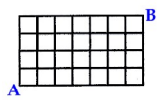
\includegraphics[scale=1.2]{kombin.PNG}
    Jika seseorang akan berjalan dari titik A ke titik B. Ada berapa banyak cara jalan terpendek 
yang dapat dipilihnya ?
    
    \item (OSP 2003) Empat pasang suami istri menonton pagelaran orkestra. Tempat duduk mereka harus 
dipisah antara kelompok suami dan kelompok istri. Untuk masing-masing kelompok disediakan 4
buah tempat duduk bersebelahan dalam satu barisan. Ada berapa banyak cara memberikan 
tempat duduk kepada mereka ?

    \item (OSK 2010) Banyaknya himpunan $X$ yang memenuhi 
$$\{1,2,\dots,1000\} \subseteq X \subseteq \{1,2,\dots,2010\}.$$

    \item (OSP 2010) Bilangan enam digit $abcdef$ dengan $a > b > c \ge d > e > f$ ada sebanyak \dots
    
    \item (OSK 2017)
	Sebuah hotel mempunyai kamar bernomor 000 sampai dengan 999. Hotel tersebut menerapkan
aturan aneh sebagai berikut: jika suatu kamar berisi tamu, dan sembarang dua digit nomor kamar
tersebut dipertukarkan tempatnya, maka diperoleh nomor kamar yang sama atau nomor kamar
yang tidak berisi tamu. Maksimal banyaknya kamar yang berisi tamu adalah \dots
\end{enumerate}

\subsection{Peluang (HOTS)}
\begin{enumerate}
            \item (OSK 2012) Suatu set soal terdiri dari 10 soal pilihan B atau S dan 15 soal pilihan ganda dengan 4 pilihan. Seorang siswa menjawab semua soal dengan menebak jawaban secara acak. Tentukan probabilitas ia menjawab dengan benar hanya 2 soal.
            
            \item (OSK 2012) Misalkan terdapat 5 kartu dimana setiap kartu diberi nomor yang berbeda yaitu 2, 3, 4, 5, 6. Kartu-kartu tersebut kemudian dijajarkan dari kiri ke kanan secara acak sehingga berbentuk barisan. Berapa probabilitas bahwa banyaknya kartu yang dijajarkan dari kiri ke kanan dan ditempatkan pada tempat ke- $i$ akan lebih besar atau sama dengan $i$ untuk setiap $i$ dengan $1 \le i \le 5$ ?
            
            \item (OSK 2013) Suatu dadu ditos enam kali. Banyak cara memperoleh jumlah mata yang muncul 28 dengan tepat satu dadu muncul angka 6 adalah \dots
            
            \item (OSK 2013) Sepuluh kartu ditulis dengan angka satu sampai sepuluh (setiap kartu hanya terdapat satu angka dan tidak ada dua kartu yang memiliki angka yang sama). Kartu - kartu tersebut dimasukkan kedalam kotak dan diambil satu secara acak. Kemudian sebuah dadu dilempar. Probabilitas dari hasil kali angka pada kartu dan angka pada dadu menghasilkan bilangan kuadrat adalah \dots
            
            \item (OSK 2018) Diberikan satu koin yang tidak seimbang. Bila koin tersebut ditos satu kali, peluang muncul angka adalah $\frac{1}{4}$. Jika ditos $n$ kali, peluang muncul tepat dua angka sama dengan peluang muncul tepat tiga angka. Nilai $n$ adalah \dots
            
            \item (OSK 2017) Pada suatu kotak ada sekumpulan bola berwarna merah dan hitam yang secara keseluruhannya kurang dari 1000 bola. Misalkan diambil dua bola. Peluang terambilnya dua bola merah adalah $p$ dan peluang terambilnya dua bola hitam adalah $q$ dengan $p-q =\frac{23}{37}$. Selisih terbesar yang mungkin dari banyaknya bola merah dan hitam adalah \dots
            
            \item (OSK 2017) Terdapat enam anak, $A, B, C, D, E$ dan $F$, akan saling bertukar kado. Tidak ada yang menerima kadonya sendiri, dan kado dari $A$ diberikan kepada $B$. Banyaknya cara membagikan kado dengan cara demikian adalah \dots
        \end{enumerate}

\end{document}


